\section{evaluation}

In this section, we evaluate the performance and scalability
of \pname against the \textit{Default-run}
(the default container startup method), \textit{Prebaking}\cite{prebaking}
(as a representative of unoptimized C/S-based container startup method)
and SEUSS\cite{seuss}.

\begin{table}
    \centering
    \caption{Test cases}
    \begin{tabular}{cccc}
        \hline
        Name               & Type                    & Language & Framework \\ \hline
        Text               & \makecell[c]{Text                              \\uploading}        & C++        & Thrift      \\
        Media              & \makecell[c]{Multimedia                        \\processing} & C++        & Thrift      \\
        ComposePost        & \makecell[c]{Database                          \\interaction}  & C++        & Thrift      \\
        UniqueID           & \makecell[c]{ID                                \\generating}         & C++        & Thrift      \\
        Timeline           & \makecell[c]{Timeline                          \\processing}   & C++        & Thrift      \\
        Decompressor       & \makecell[c]{Online                            \\decompressor}     & Golang     & Beego       \\
        Meme               & \makecell[c]{Image                             \\processing}        & JavaScript & Express     \\
        Inception          & \makecell[c]{Image                             \\classification}   & Python   & Flask       \\
        Sentiment-analysis & \makecell[c]{Sentiment                         \\analysis}      & Python   & Flask       \\
        Search             & \makecell[c]{Data                              \\retrieval}          & Java     & Spring boot \\ \hline
    \end{tabular}
    \label{table:test-case}
\end{table}

The serverless function test cases used in this section are shown in the table \ref{table:test-case}. 
Half of the test cases are derived from the \textit{Social Network} application in the 
microservice application set DeathStar\cite{deathstar}. 
The selected container service names are Text, Media, ComposePost, UniqueID, and Timeline; 
the other half of the test cases are serverless 
computing applications constructed in this paper based on different languages and development frameworks.

We use an x86-64 machine (the experimental machine) with 
an 8-core Intel i7-9700 CPU, 128GB memory and Samsung
1TB SSD, to evaluate our system. 
The OS is Ubuntu 18.04 with Linux kernel 5.8.9.

The experiment in this section is divided into three parts. 
The first part mainly verifies the optimization 
effect of our system in terms of serverless function startup latency. 
The verification method is to use all the systems under test 
to start multiple different types of serverless functions and record the function startup latency. 
The experiment will be performed multiple times to obtain the average startup latency of the function.
The second part of the experiment verifies the optimization effect of this system on the memory occupancy during deployment of serverless functions. 
The experiment use systems to start a certain number of serverless functions in each test cycle, 
wait for all functions to start and use related tools to record the memory usage of all functions. 
The third part of the experiment is to test 
the concurrent function deployment performance of the system. 
The verification method is to perform large-scale 
concurrent deployment of serverless functions on the experimental node.

\subsection{Function Startup Latency}

\begin{figure*}[t]
    \centering
    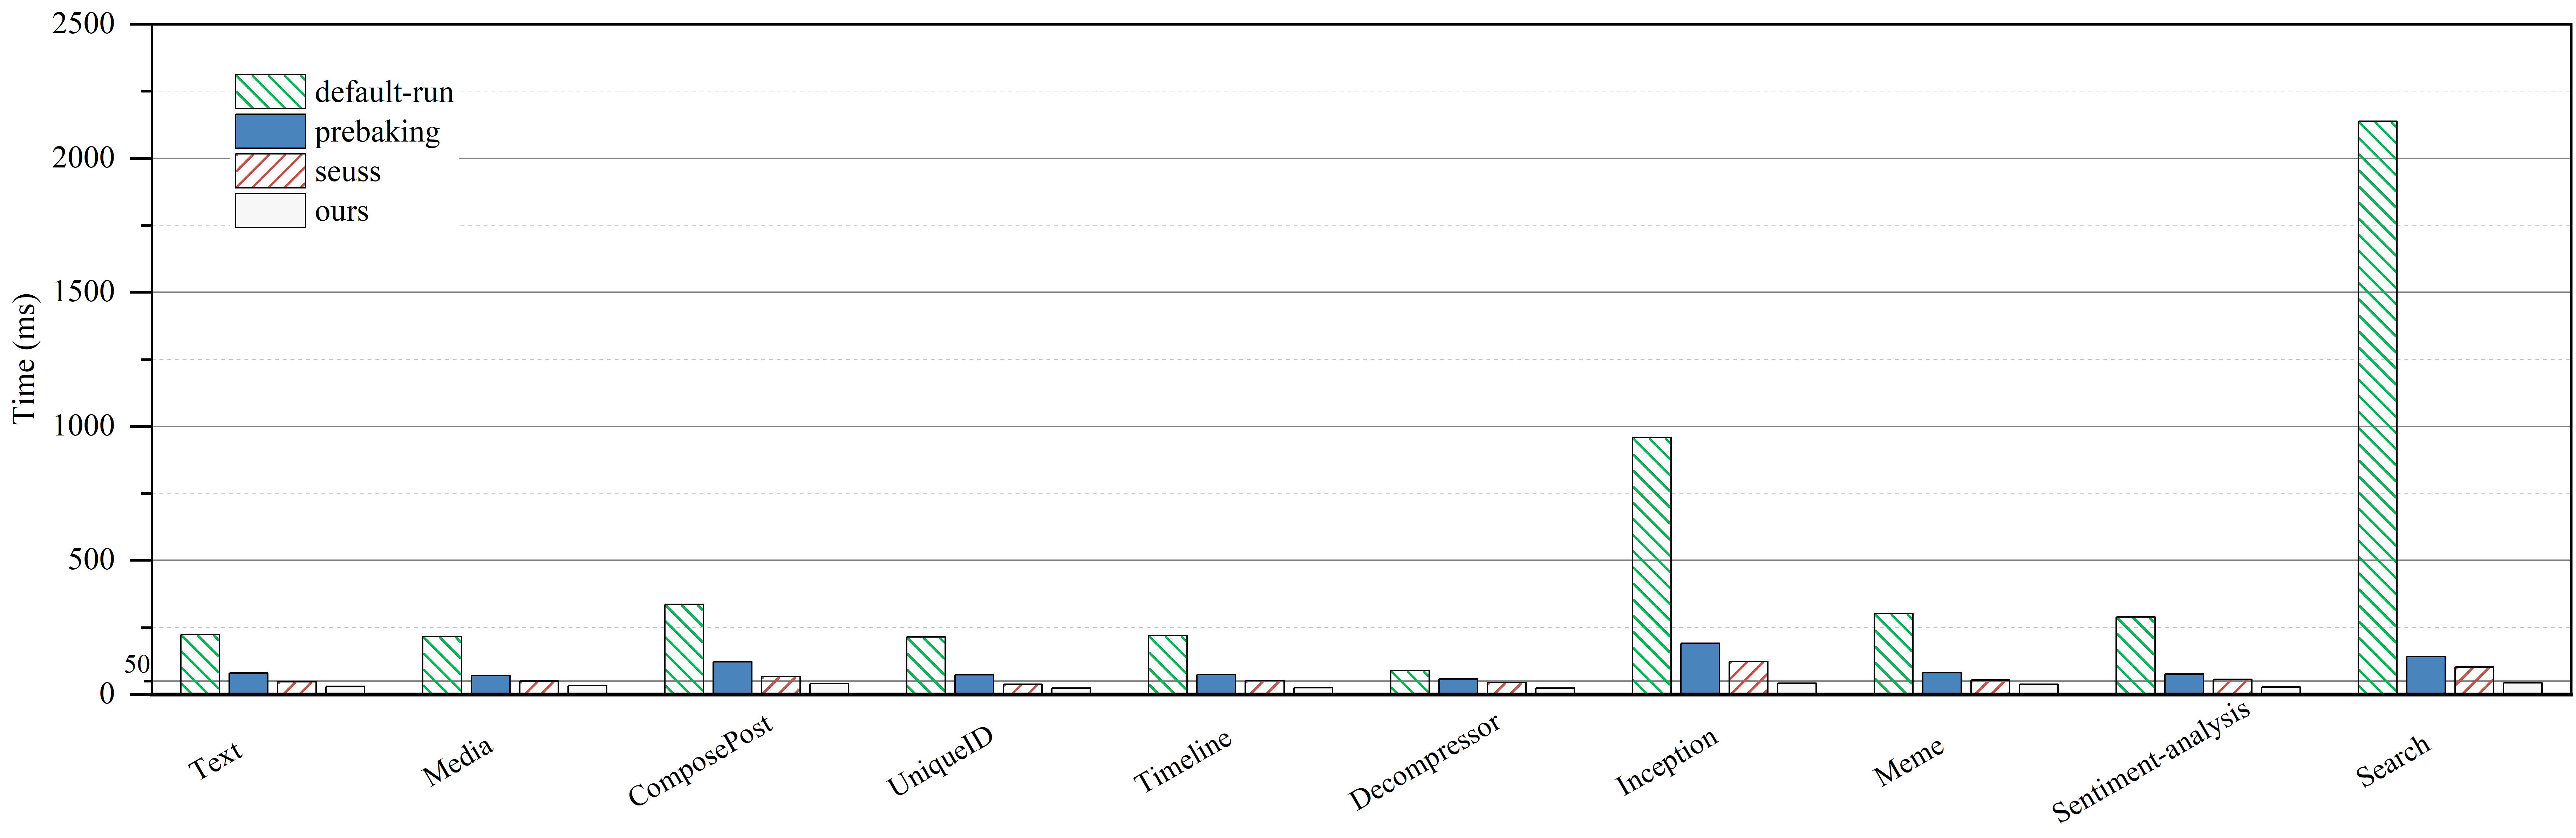
\includegraphics[width=\linewidth]{images/startup-latency.png}
    \caption{Startup latency of serverless functions}
    \label{startup-latency}
\end{figure*}

For \pname, \textit{default-run} and \textit{prebaking}, 
the startup latency on the work node is defined as the time 
interval from the time the runc component receives the request 
to start the serverless function to the time that the 
serverless function is able to handle the coming request; 
for the \textit{seuss}, it is the time interval from when the Rumprun 
system receives the instruction to start the 
serverless function to when the serverless function is started and can accept the request.

The result of the experiment is shown in Figure \ref{startup-latency}. 
The result shows that the serverless function isolation environment pooling strategy and the memory mapping strategy adopted 
in this paper can effectively reduce the function startup latency. 
The startup latency can be reduced by at least 30\% compared to other systems, 
and at least 70\% when compared to the \textit{default-run}.
In addition, the startup latency of all test cases starting by \pname is below 50 milliseconds.

After analyzing the optimized startup phase, 
it can be seen that the isolation environment 
pooling strategy reduces the time spent in the 
isolation environment initialization stage from 
tens of milliseconds to a few milliseconds, 
and the memory mapping strategy also reduces the time spent 
in the memory loading stage to about ten milliseconds.

\subsection{Memory Occupation}

The experiment of the memory occupation uses systems to deploy 
different types of serverless functions, 
and the number of copies of each type of serverless function is 10, 
and the amount of memory used by each function is collected to 
obtain the total amount of memory occupied by all serverless functions of each type.

\begin{figure*}[t]
    \centering
    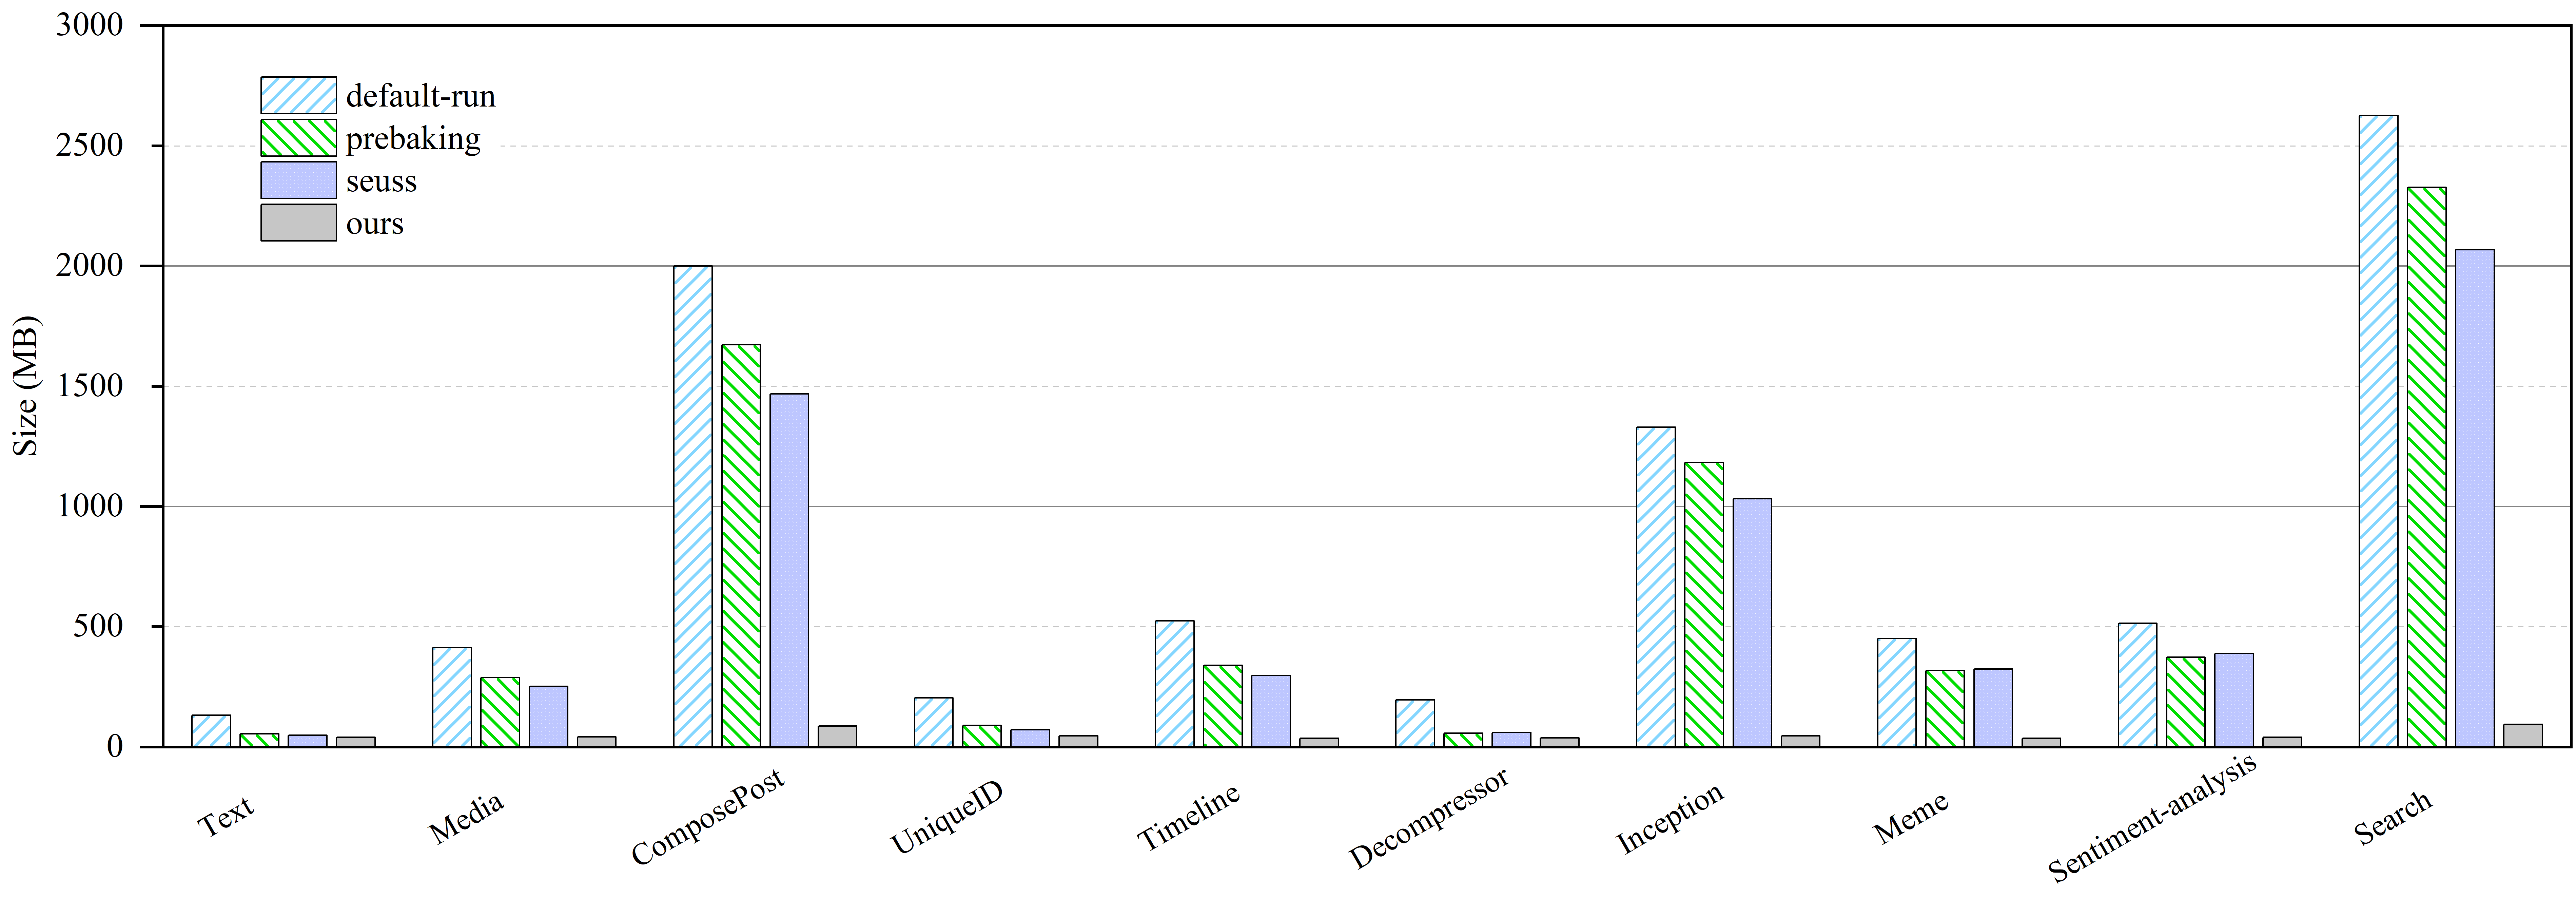
\includegraphics[width=\linewidth]{images/memory.png}
    \caption{Memory footprint of multiple serverless functions}
    \label{memory}
\end{figure*}

The test result(figure \ref{memory}) shows that the use of function memory 
sharing mapping strategy can effectively reduce the resource 
occupation of serverless functions. 
Compared with other systems, 
the total memory occupied by the serverless functions 
deployed by our system is reduced by 20\% to 90\%. 
There is a lot of redundancy in the memory data of the serverless function deployed by other systems, 
but due to the natural isolation between the virtual memory spaces of the process, data cannot be shared, 
resulting in a waste of memory resources.

\subsection{Concurrent Deployment of Serverless Functions}

\begin{figure}[t]
    \centering
    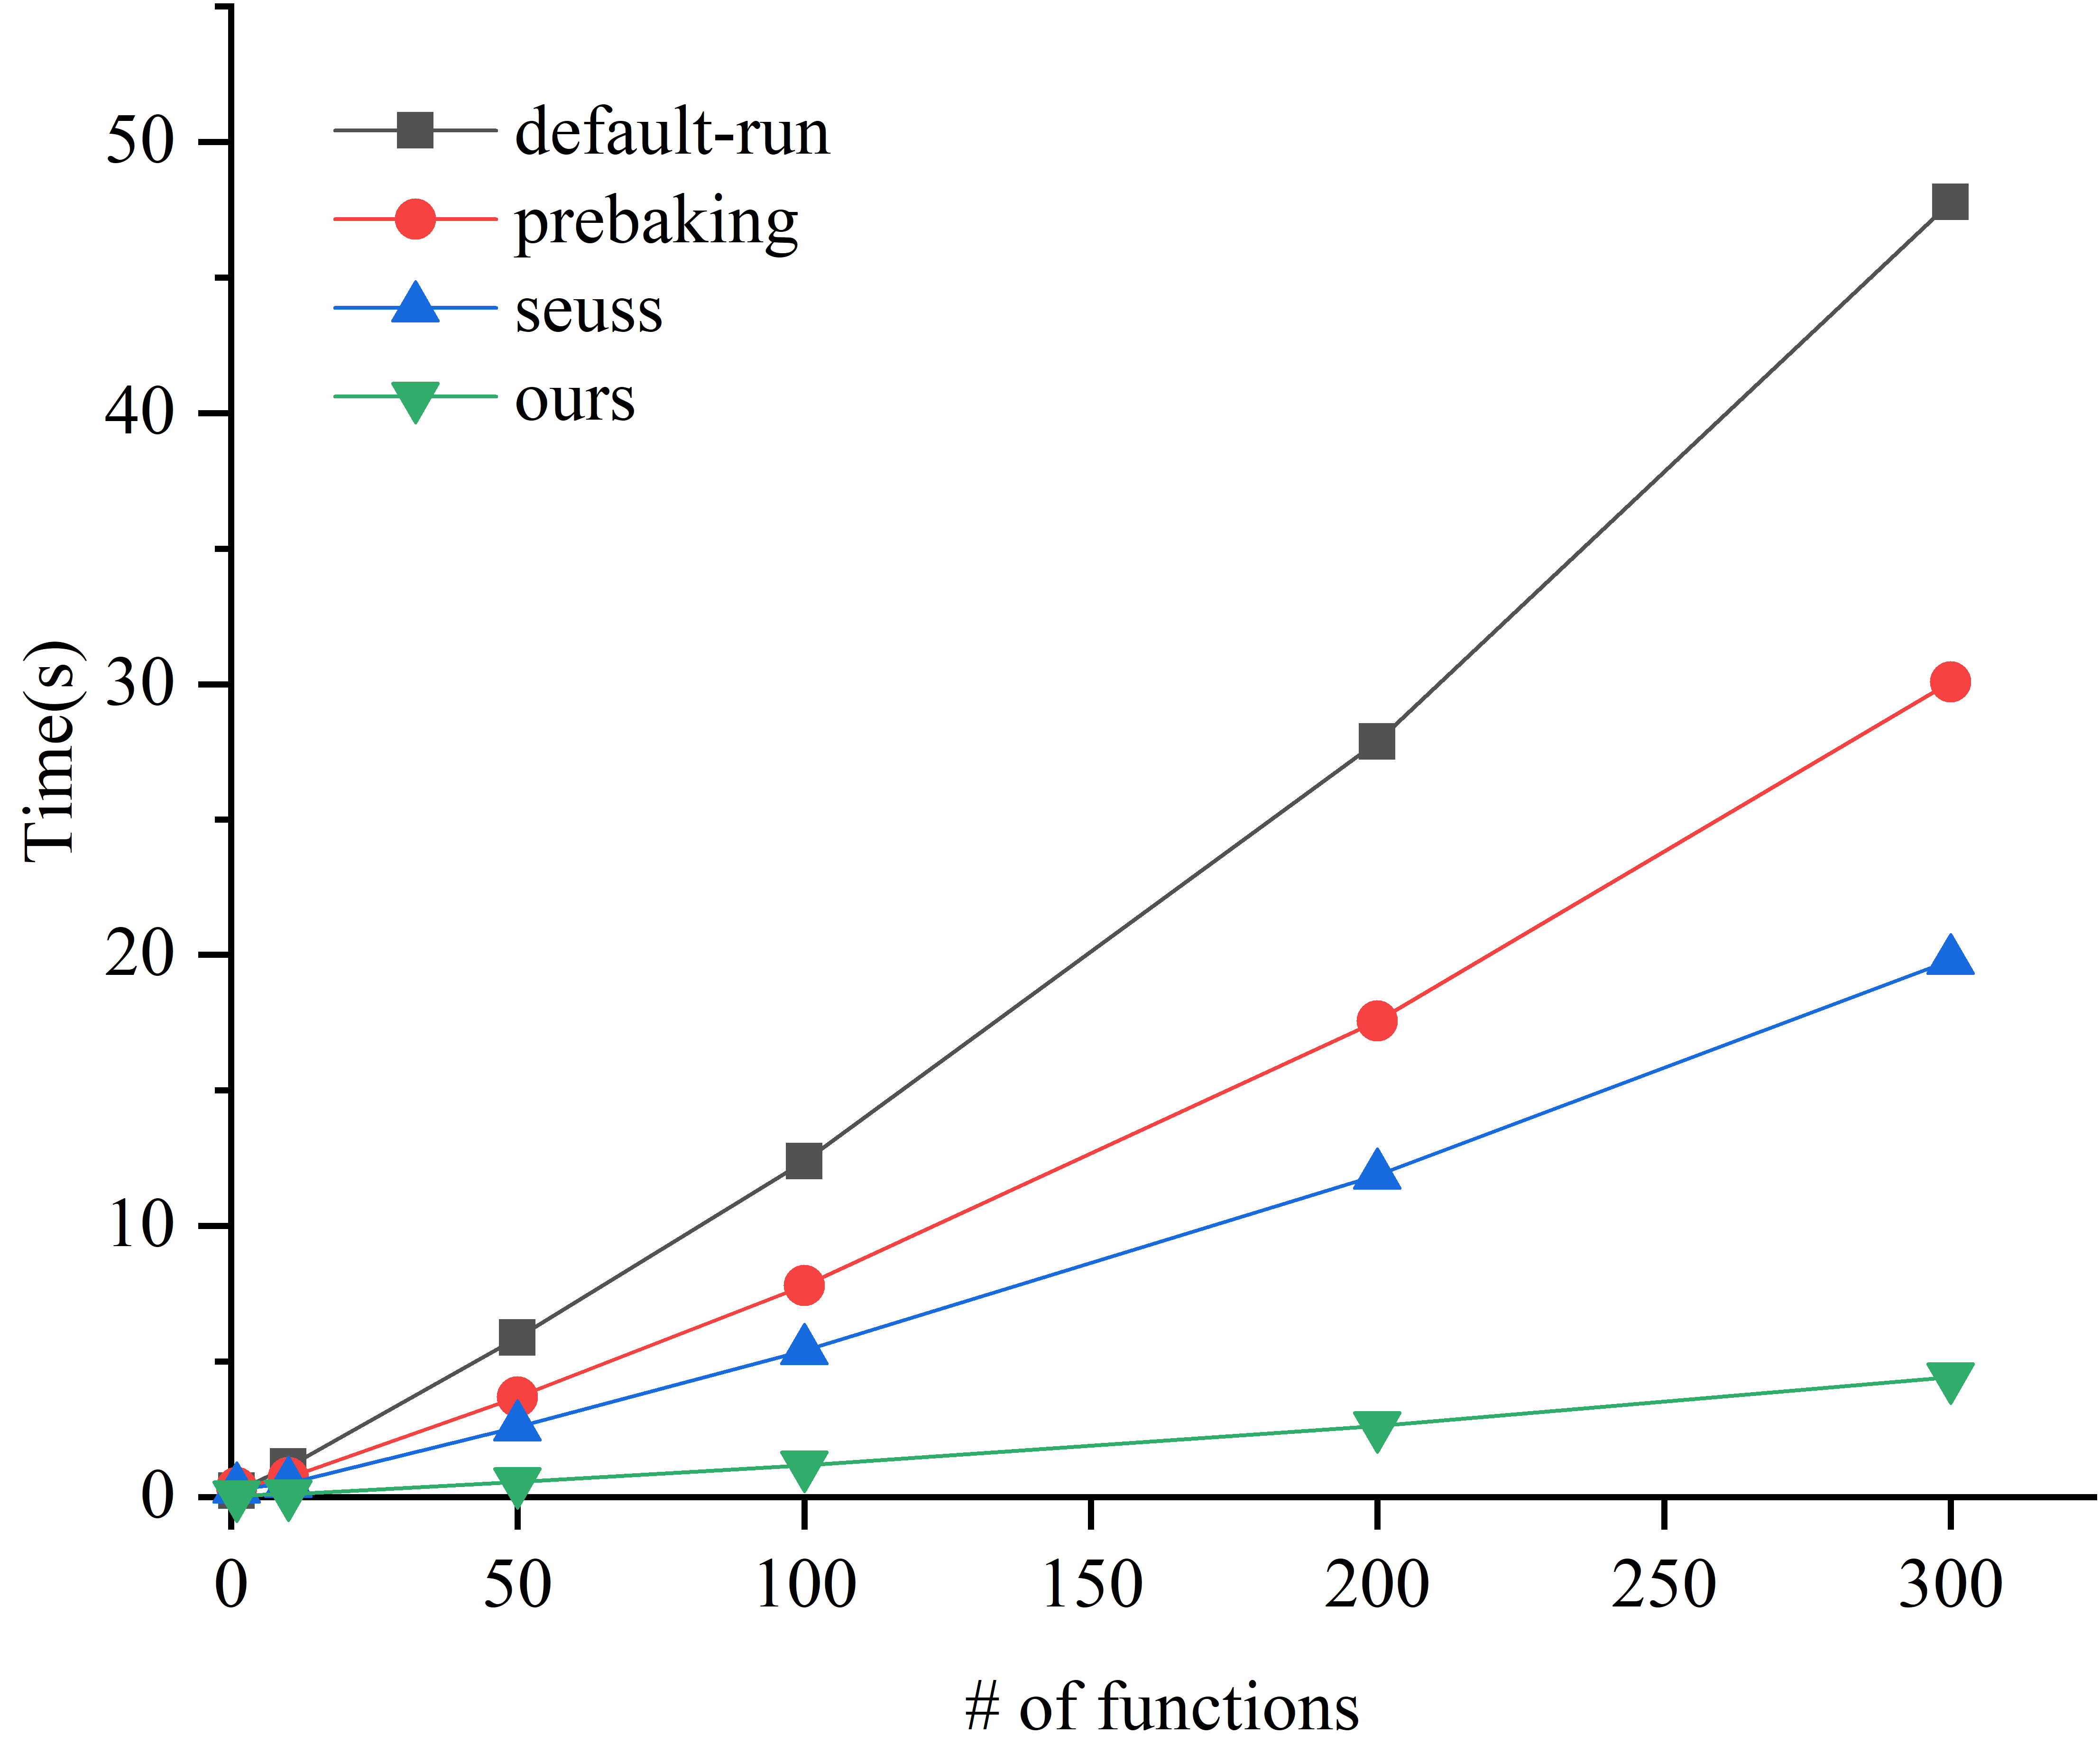
\includegraphics[width=\linewidth]{images/concurrent.png}
    \caption{Latency of current deployment}
    \label{concurrent}
\end{figure}

This experiment uses all systems to deploy serverless functions at a concurrency of 1, 10, 50, 100, 200, and 300. 
The used test cases and their deployment ratio are randomly generated, 
The experimental results are shown in Figure \ref{concurrent}. 
The result shows that compared with the \textit{default-run}, 
our system can save up to 90\% of the deployment time. 
Even compared with other systems, 
the deployment efficiency of our system under high concurrency is also very advantageous. 
This is due to the use of C/S technique to accelerate the startup of serverless functions, at the same time, 
the isolate environment pooling strategy 
and the memory sharing mapping strategy
are adapted to greatly reduce the startup latency. 
In general, 
our system does not have a explosive growth in deployment 
time while the number of functions increases, 
which is conducive to the serverless computing platform to provide services more quickly and efficiently.
